\documentclass{article}

\usepackage{fancyhdr}
\usepackage{extramarks}
\usepackage{amsmath}
\usepackage{amsthm}
\usepackage{amsfonts}
\usepackage{tikz}
\usepackage[plain]{algorithm}
\usepackage{algpseudocode}
\usepackage{indentfirst}


\usetikzlibrary{automata,positioning}

%
% Basic Document Settings
%

\topmargin=-0.45in
\evensidemargin=0in
\oddsidemargin=0in
\textwidth=6.5in
\textheight=9.0in
\headsep=0.25in

\linespread{1.1}

\pagestyle{fancy}
\lhead{\hmwkAuthorName}
%\hmwkClassInstructor\
\chead{\hmwkClass\ (\hmwkClassTime): \hmwkTitle}
\rhead{\firstxmark}
\lfoot{\lastxmark}
\cfoot{\thepage}

\renewcommand\headrulewidth{0.4pt}
\renewcommand\footrulewidth{0.4pt}

\setlength\parindent{0pt}

%
% Create Problem Sections
%

\newcommand{\enterProblemHeader}[1]{
    \nobreak\extramarks{}{Problem \arabic{#1} continued on next page\ldots}\nobreak{}
    \nobreak\extramarks{Problem \arabic{#1} (continued)}{Problem \arabic{#1} continued on next page\ldots}\nobreak{}
}

\newcommand{\exitProblemHeader}[1]{
    \nobreak\extramarks{Problem \arabic{#1} (continued)}{Problem \arabic{#1} continued on next page\ldots}\nobreak{}
    \stepcounter{#1}
    \nobreak\extramarks{Problem \arabic{#1}}{}\nobreak{}
}

\setcounter{secnumdepth}{0}
\newcounter{partCounter}
\newcounter{homeworkProblemCounter}
\setcounter{homeworkProblemCounter}{1}
\nobreak\extramarks{Problem \arabic{homeworkProblemCounter}}{}\nobreak{}

%
% Homework Problem Environment
%
% This environment takes an optional argument. When given, it will adjust the
% problem counter. This is useful for when the problems given for your
% assignment aren't sequential. See the last 3 problems of this template for an
% example.
%
\newenvironment{homeworkProblem}[1][-1]{
    \ifnum#1>0
        \setcounter{homeworkProblemCounter}{#1}
    \fi
    \section{Problem \arabic{homeworkProblemCounter}}
    \setcounter{partCounter}{1}
    \enterProblemHeader{homeworkProblemCounter}
}{
    \exitProblemHeader{homeworkProblemCounter}
}

%
% Homework Details
%   - Title
%   - Due date
%   - Class
%   - Section/Time
%   - Instructor
%   - Author
%

\newcommand{\hmwkTitle}{Homework\ \#1}
\newcommand{\hmwkDueDate}{Jan.25, 2022}
\newcommand{\hmwkClass}{EECS545}
\newcommand{\hmwkClassTime}{Section001}
\newcommand{\hmwkClassInstructor}{Instructor:Honglak Lee}
\newcommand{\hmwkAuthorName}{\textbf{Tiejin Chen}}


%
% Title Page
%

\title{
    \vspace{2in}
    \textmd{\textbf{\hmwkClass(\hmwkClassTime):\  \hmwkTitle}}\\
    \normalsize\vspace{0.1in}\small{Due\ on\ \hmwkDueDate\ at 11:59pm}\\
    \vspace{0.1in}\large{\textit{\hmwkClassInstructor\ }}
    \vspace{3in}
}

\author{\hmwkAuthorName \and \textbf{tiejin@umich.edu}}
\date{}
\renewcommand{\part}[1]{\textbf{\large Part \Alph{partCounter}}\stepcounter{partCounter}\\}

%
% Various Helper Commands
%

% Useful for algorithms
\newcommand{\alg}[1]{\textsc{\bfseries \footnotesize #1}}

% For derivatives
\newcommand{\deriv}[1]{\frac{\mathrm{d}}{\mathrm{d}x} (#1)}

% For partial derivatives
\newcommand{\pderiv}[2]{\frac{\partial}{\partial #1} (#2)}

% Integral dx
\newcommand{\dx}{\mathrm{d}x}

% Alias for the Solution section header
\newcommand{\solution}{\textbf{\large Solution}}

% Probability commands: Expectation, Variance, Covariance, Bias
\newcommand{\E}{\mathrm{E}}
\newcommand{\Var}{\mathrm{Var}}
\newcommand{\Cov}{\mathrm{Cov}}
\newcommand{\Bias}{\mathrm{Bias}}

\begin{document}

\maketitle

\pagebreak
\setlength{\parindent}{2em}

\begin{homeworkProblem}
\textbf{(a)}\\
We have:
\[L_1(w) = \sum_{i=1}^n y^{(i)}log(h(x^{(i)})) = y^{(i)}log((1+e^{-w^Tx^{(i)}})^{-1}) = -y^{(i)}log(1+e^{-w^Tx^{(i)}}) \]
\[L_2(w) = \sum_{i=1}^n (1-y^{(i)})log(1-h(x^{(i)})) = (1-y^{(i)})log(\frac{e^{-w^Tx^{(i)}}}{1+e^{-w^Tx^{(i)}}}) = (1-y^{(i)})[-w^Tx^{(i)}-log(1+e^{-w^Tx^{(i)}})] \]
Wa assumed $w=(w_1,...,w_p), x^{(i)} = (x_{i1},...,x_{ip})$
\[\frac{\partial L_1(w)}{\partial w_j} =\sum_{i=1}^n (1-h(x^{(i)}))x_{ij}y^{(i)} \]
\[\frac{\partial L_2(w)}{\partial w_j} = -\sum_{i=1}^n   h(x^{(i)})x_{ij}(1-y^{(i)})\]
 Thus, 
\[\frac{\partial L(w)}{\partial w_j} = \sum_{i=1}^n (y^{(i)}-h(x^{(i)}))x_{ij} \]
Hence, we can get:
\[\frac{\partial L(w)}{\partial w_j \partial w_m} = -\sum_{i=1}^n\frac{e^{-w^Tx^{(i)}}}{(1+e^{-w^Tx^{(i)}})^2} x_{ij}x_{im} \]
We can get the Hessian matrix:
\[H = X^TDX\]
Where $X =(x_1,...,x_n)^T$ is a $n \times p$ matrix. And D is a diagonal matrix where $D_{ii}=-\frac{e^{-w^Tx^{(i)}}}{(1+e^{-w^Tx^{(i)}})^2}$.

Now we prove it is negative semi-definite.We consider for any $z$ which is $p \times 1$ vector to get:
\[z^THz = z^TX^TDXz = (Xz)^TD(Xz) \]
We know $Xz$ is a $n \times 1$ vector. We assumed  $Xz = (f_1,...,f_n)$. Then since $D$ is a diagonal matrix, we have:
\[(Xz)^TD(Xz) = \sum_{i=1}^n D_{ii}f_i^2 \]
We know that $D_{ii}=-\frac{e^{-w^Tx^{(i)}}}{(1+e^{-w^Tx^{(i)}})^2} <0, f_i^2 \geq 0, D_{ii}f_i^2 \leq 0$. Thus we can get:
\[z^THz = (Xz)^TD(Xz) \leq 0 \]
Which is the end of our proof.

\textbf{(b)}\\
In this problem, we aim to maximize the log likelihood function, which means we need to minimize the negtive log likelihood function:
\[-l(w) = -\sum_{i=1}^n y^{(i)}log(h(x^{(i)}))+(1-y^{(i)})log(1-h(x^{(i)})) \]
We can get:
\[\frac{\partial -l(w)}{\partial w} = -\frac{\partial l(w)}{\partial w}\]
\[\frac{\partial -l(w)}{\partial w_i\partial w_j} = -\frac{\partial l(w)}{\partial w_i\partial w_j}\]
Thus let $H^*$ presents the Hessian matrix of $-l(w)$, we have $H^*=-H$. Thus,the newton method is:
\[w_{(t)} = w_{(t-1)} - (-H)^{-1}\frac{\partial -l(w)}{\partial w} =  w_{(t-1)}-H^{-1}\frac{\partial l(w)}{\partial w} \]
Here, $w_{(t)}$ is a vector presents the t-times updated weight $w$.

We get the result that after 5 epoches, logistic regression converges. And we get the parameter is:
\[w_b = -1.84922892, w_1 = -0.62814188,w_2 = 0.85846843\]
where $w_b$ is the intercept term.

\textbf{(c)}\\
We get the plot:
\begin{figure}[H]
\centering
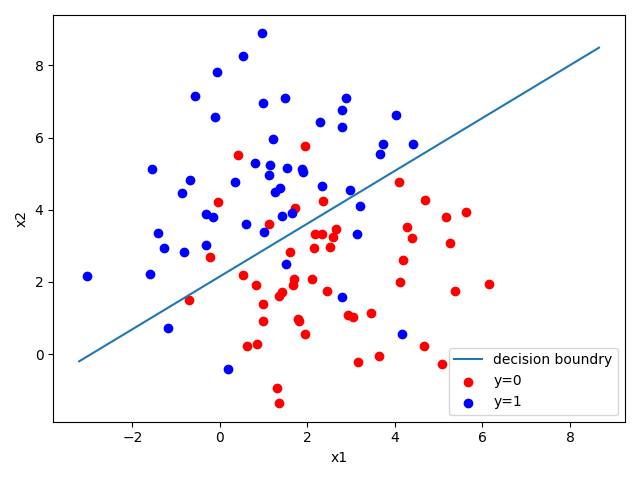
\includegraphics[scale=0.7]{images/1.png}
\end{figure}
\end{homeworkProblem}

\begin{homeworkProblem}
\textbf{(a)}\\
We can assume$w_K=(0,..,0)$ is a zero vector. Then we can use $p(y=K|x,w) = \frac{exp(w_K^T\phi(x))}{1+\sum_{j=1}^{K-1} exp(w_j^T\phi(x))}$.Let us first consider $\sum_{k=1}^K log([p(y^{(i)}=k|x^{(i)},w)]^{I({y^{(i)}=k})})$. We have:
\[\sum_{k=1}^K log([p(y^{(i)}=k|x^{(i)},w)]^{I({y^{(i)}=k})}) = \sum_{k=1}^K I({y^{(i)}=k})log(p(y^{(i)}=k|x^{(i)},w)) \]
for any term that $k \neq m$, we have:
\[\frac{\partial I({y^{(i)}=k})log(p(y^{(i)}=k|x^{(i)},w))}{\partial w_m} = -I({y^{(i)}=k})\frac{exp(w_m^T\phi(x^{(i)}))}{1+\sum_{j=1}^{K-1}exp(w_j^T\phi(x^{(i)}))} \]

If we have $k = m$, then we have:
\[\frac{\partial I({y^{(i)}=m})log(p(y^{(i)}=m|x^{(i)},w))}{\partial w_m}=I({y^{(i)}=m})\frac{1+\sum_{j \neq m,j\leq K-1}exp(w_j^T\phi(x^{(i)}))}{1+\sum_{j=1}^{K-1}exp(w_j^T\phi(x^{(i)}))} \]

Hence, we can see that, if $y^{(i)}\neq m$, then only term left is one of $\frac{\partial I({y^{(i)}=k})log(p(y^{(i)}=k|x^{(i)},w))}{\partial w_m}$. if $y^{(i)}= m$, the only term left is $\frac{\partial I({y^{(i)}=m})log(p(y^{(i)}=m|x^{(i)},w))}{\partial w_m}$. Thus we have:
\[\frac{\partial \sum_{k=1}^K I({y^{(i)}=k})log(p(y^{(i)}=k|x^{(i)},w))}{\partial w_m} = -\frac{exp(w_m^T\phi(x^{(i)}))}{1+\sum_{j=1}^{K-1}exp(w_j^T\phi(x^{(i)}))},y^{(i)}\neq m\]

\[\frac{\partial \sum_{k=1}^K I({y^{(i)}=k})log(p(y^{(i)}=k|x^{(i)},w))}{\partial w_m} =\frac{1+\sum_{j \neq m,j\leq K-1}exp(w_j^T\phi(x^{(i)}))}{1+\sum_{j=1}^{K-1}exp(w_j^T\phi(x^{(i)}))}, y^{(i)}= m \]
We can write this formula as:
\[\frac{\partial \sum_{k=1}^K I({y^{(i)}=k})log(p(y^{(i)}=k|x^{(i)},w))}{\partial w_m} = \phi(x^{(i)})[I({y^{(i)}=m})-\frac{exp(w_m^T\phi(x^{(i)}))}{1+\sum_{j=1}^{K-1}exp(w_j^T\phi(x^{(i)}))}] \]
Thus, we have:
\[\nabla_{w_m}l(w) = \sum_{i=1}^N\phi(x^{(i)})[I({y^{(i)}=m})-\frac{exp(w_m^T\phi(x^{(i)}))}{1+\sum_{j=1}^{K-1}exp(w_j^T\phi(x^{(i)}))}] \]
which is the end of our proof. And the gradient ascent update will be:
\[w_m^* \leftarrow w_m^* +\alpha \nabla_{w_m}l(w) \]
for $m=1..,K-1$,where $\nabla_{w_m}l(w)$ is
\[\sum_{i=1}^N\phi(x^{(i)})[I({y^{(i)}=m})-\frac{exp(w_m^T\phi(x^{(i)}))}{1+\sum_{j=1}^{K-1}exp(w_j^T\phi(x^{(i)}))}] = \sum_{i=1}^N\phi(x^{(i)})[I({y^{(i)}=m})-p(y^{(i)}=m|x^{(i)},w)] \]

\textbf{(b)}\\
We set initial of $w$ is all zero. And after 300 epoches training with learning rate 0.0005, we get the accuracy of test set is 0.94.

\end{homeworkProblem}

\begin{homeworkProblem}
\textbf{(a)}\\
By Bayesian's theroem, we have:
\[P(y=1|x) = \frac{p(x|y=1)p(y=1)}{p(x)} = \frac{p(x|y=1)p(y=1)}{p(x|y=0)p(y=0)+p(x|y=1)p(y=1)} = \frac{1}{1+\frac{p(x|y=0)p(y=0)}{p(x|y=1)p(y=1)}}\]
Now we only need to consider $\frac{p(x|y=0)p(y=0)}{p(x|y=1)p(y=1)}$.We can have:
\[\frac{p(x|y=0)p(y=0)}{p(x|y=1)p(y=1)} = \frac{1-\phi}{\phi}\frac{exp(-\frac{1}{2}(x_i-\mu_0)^T \Sigma^{-1}(x_i-\mu_0))}{exp(-\frac{1}{2}(x_i-\mu_1)^T \Sigma^{-1}(x_i-\mu_1))} \]
We take log function to $\frac{p(x|y=0)p(y=0)}{p(x|y=1)p(y=1)}$ to get:
\[log(\frac{p(x|y=0)p(y=0)}{p(x|y=1)p(y=1)}) = log(\frac{1-\phi}{\phi})+ (\mu_0-\mu_1)^T\Sigma^{-1}x_i +\frac{1}{2}(\mu_1-\mu_0)^T\Sigma^{-1}(\mu_1-\mu0) \]
We consider $x_i^* = (1,x_i^T)^T, w=(log(\frac{1-\phi}{\phi})+\frac{1}{2}(\mu_1-\mu_0)^T\Sigma^{-1}(\mu_1-\mu0),(\mu_0-\mu_1)^T\Sigma^{-1})^T$. Then we have:
\[log(\frac{p(x|y=0)p(y=0)}{p(x|y=1)p(y=1)}) = w^Tx_i^* \to frac{p(x|y=0)p(y=0)}{p(x|y=1)p(y=1)} = exp(w^Tx_i^*) \]
Thus, we can get:
\[P(y=1|x) = \frac{1}{1+exp(w^Tx_i^*)} \]
Which is the end of our proof.

\textbf{(b)}\\
We can rewrite the $p(x_i|y_i) =p(x_i|y_i=0)^{1-y_i}p(x_i|y_i=1)^{y_i}$.Hence we can get:

\[L(\phi,\mu_0,\mu_1,\Sigma) = \prod_{i=1}^N [p(x_i|y_i=0)(1-\phi)]^{1-y_i}[p(x_i|y_i=1)\phi]^{y_i} \]
Then we take log function to get:
\begin{equation*}
\begin{aligned}
l(\phi,\mu_0,\mu_1,\Sigma) 
&= \sum_{i=1}^N (1-y_i)log[p(x_i|y_i=0)(1-\phi)] +y_ilog[p(x_i|y_i=1)\phi] \\
&= \sum_{i=1}^N (1-y_i)[log(1-\phi)-\frac{1}{2}log(2\pi\sigma^2)-\frac{(x_i-\mu_0)^2}{2\sigma^2}]\\
&+y_i[log(\phi)-\frac{1}{2}log(2\pi\sigma^2)-\frac{(x_i-\mu_1)^2}{2\sigma^2}]
\end{aligned}
\end{equation*}

Then we have:
\[\frac{\partial l}{\partial \phi} = \frac{1}{\phi}\sum_{i=1}^N y_i - \frac{1}{1-\phi}\sum_{i=1}(1-y_i) = 0 \]
\[\frac{\partial l}{\partial \mu_0} = \sum_{i=1}^N\frac{x_i-\mu_0}{\sigma^2}(1-y_i) = 0 \to \sum_{i=1}^N(x_i-\mu_0)(1-y_i) = 0\]
\[\frac{\partial l}{\partial \mu_1} = \sum_{i=1}^N\frac{x_i-\mu_1}{\sigma^2} y_i = 0 \to \sum_{i=1}^N(x_i-\mu_1) y_i = 0\]
\[\frac{\partial l}{\partial \sigma^2} = \frac{\sum_{i=1}^N(1-y_i)(x_i-\mu_0)^2}{2\sigma^4}+\frac{\sum_{i=1}^N y_i(x_i-\mu_1)^2}{2\sigma^4}-\frac{N}{2\sigma^2} = 0  \]

We know $y_i = I(y_i=1), 1-y_i = I(y_i=0)$. And we can get the MLE of all four parameter is:
\[\hat{\phi} = \frac{\sum_{i=1}^N y_i}{N} = \frac{1}{N}sum_{i=1}^NI(y_i=1)\]
\[\hat{\mu_0} = \frac{\sum_{i=1}^N I(y_i=0)x_i}{\sum_{i=1}^N I(y_i=0)} \]
\[\hat{\mu_1} = \frac{\sum_{i=1}^N I(y_i=1)x_i}{\sum_{i=1}^N I(y_i=1)} \]
\[\hat{\sigma^2} = \frac{1}{N}\sum_{i=1}^N(x_i-\mu_{y_i})^2 = \frac{1}{N}\sum_{i=1}^N(x_i-\mu_{y_i})(x_i-\mu_{y_i})^T \]
which is the end of our proof.

\textbf{(c)}\\

From part(b), we know:
\begin{equation*}
\begin{aligned}
l(\phi,\mu_0,\mu_1,\Sigma) 
&= \sum_{i=1}^N (1-y_i)log[p(x_i|y_i=0)(1-\phi)] +y_ilog[p(x_i|y_i=1)\phi] \\
&= \sum_{i=1}^N (1-y_i)[log(1-\phi)-\frac{1}{2}log(2\pi|\Sigma|)-\frac{1}{2}(x-\mu_0)^T\Sigma^{-1}(x-\mu_0)]\\
&+y_i[log(\phi)-\frac{1}{2}log(2\pi|\Sigma|)-\frac{1}{2}(x-\mu_1)^T\Sigma^{-1}(x-\mu_1)]
\end{aligned}
\end{equation*}



And we know:
\[\frac{\partial l}{\partial \phi} = \frac{1}{\phi}\sum_{i=1}^N y_i - \frac{1}{1-\phi}\sum_{i=1}(1-y_i) = 0 \]
For $\mu_0$, we have:
\[(x_i-\mu_0)^T \Sigma^{-1}(x_i-\mu_0) = x_i^T \Sigma^{-1}x_i -x_i^T\Sigma^{-1}\mu_0- \mu_0^T\Sigma^{-1}x_i +\mu_0^T \Sigma^{-1} \mu_0\]
\[\frac{d^TA}{\partial d} = A,\frac{Ad}{\partial d} = A^T, \frac{d^TAd}{\partial d} = (A+A^T)d\]
\[\frac{\partial (x_i-\mu_0)^T \Sigma^{-1}(x_i-\mu_0)}{\partial \mu_0} = -\Sigma^{-T}x_i -\Sigma^{-1}x_i+(\Sigma^{-T}+\Sigma^{-1})\mu_0 \]
Since we know $\Sigma$ is corvaiance matrix and thus it is symmetric. Hence we have:
\[\frac{\partial l}{\partial \mu_0} = \Sigma^{-1}\sum_{i=1}^N (1-y_i)(x_i-\mu_0) = 0 \to \sum_{i=1}^N (1-y_i)(x_i-\mu_0) = 0\]
$\mu_1$ is similar, we have:
\[\frac{\partial l}{\partial \mu_1} = \Sigma^{-1}\sum_{i=1}^N y_i(x_1-\mu_1) = 0 \to \sum_{i=1}^N y_1(x_i-\mu_1) = 0\]

Thus, we can get MLE for three parameter are:
\[\hat{\phi} = \frac{\sum_{i=1}^N y_i}{N} = \frac{1}{N}sum_{i=1}^NI(y_i=1)\]
\[\hat{\mu_0} = \frac{\sum_{i=1}^N I(y_i=0)x_i}{\sum_{i=1}^N I(y_i=0)} \]
\[\hat{\mu_1} = \frac{\sum_{i=1}^N I(y_i=1)x_i}{\sum_{i=1}^N I(y_i=1)} \]
which is the end of our proof.
\end{homeworkProblem}



\begin{homeworkProblem}
\textbf{(a)}\\
We use log function to prevent the very small numbers problem. And we get the error in test set is 1.6250\%

\textbf{(b)}\\
We know:
\[log(\frac{p(x_j=i|y=1)}{p(x_j=i|y=0)}) = log(p(x_j=i|y=1)) - log(p(x_j=i|y=0)) \]
And we can get 5 tokens that are most indicative of the SPAM are:['httpaddr', 'spam', 'unsubscrib', 'ebai', 'valet']


\textbf{(c)}\\
We can get the plot.
\begin{figure}[H]
\centering
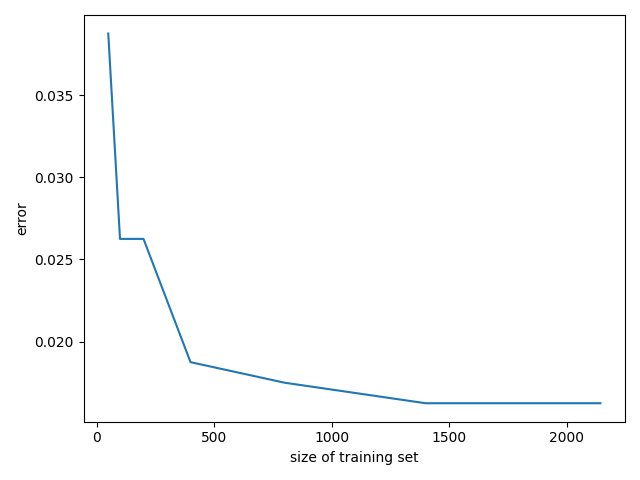
\includegraphics[scale=0.7]{images/2.png}
\end{figure}

And we find that more trianing set size give us better classification error. And when training size is 1400, it gives us the best classification error and the error is same as using whole training set.


\end{homeworkProblem}
\end{document}
